% Vzor DP1/BP1
% 30-Apr-14

\documentclass[11pt,slovak,a4paper]{article}
%\usepackage[T1]{fontenc}
\usepackage[IL2]{fontenc}
\usepackage[cp1250]{inputenc}
\usepackage{babel}
\usepackage{url}
\usepackage[nottoc]{tocbibind}
\usepackage{fancyhdr}
\usepackage{ifthen}
\usepackage{hyperref}
\usepackage{graphicx}
\usepackage{listings}
\lstset{language=[AspectJ]Java,basicstyle=\fontsize{9}{10.8}\selectfont,showstringspaces=false,columns=fullflexible}

\newcommand{\magnf}{.65}
\newcommand{\codesize}{\footnotesize}
\newcommand{\lsti}{\ajset\lstinline[basicstyle=\fontsize{10}{12}\selectfont]}
\newcommand{\emp}[1]{\emph{#1}}
\newcommand{\ffe}[1]{\textsf{#1}}

% bal�k listings niekedy niektor� k���ov� slov� nezv�raz�uje ak to nedostane pr�kazom tesne pred textom
\newcommand{\ajset}{\lstset{emph={class,aspect,new,call,execution,set,int,advice,public,thisJoinPointStaticPart,thisEnclosingJoinPointStaticPart,@annotation,dominates},emphstyle=\bfseries}}

\pagestyle{myheadings}

\begin{document}

\input title.lx

\begin{titlepage}
\section*{Anot�cia}
\ldots
\end{titlepage}


\tableofcontents


\pagestyle{fancy}
\headheight 14pt

\section{�vod} \label{in}

\ldots



\section{Nejak� �as�} \label{nejaka}

\ldots

\subsection{Pod�as�} \label{nejaka-pod}

\ldots


\subsection{�al�ia pod�as�} \label{nejaka-dalsia}

Na obr�zku~\ref{f:gen-spec} vid�me\ldots

\begin{figure}[tbh] \centering
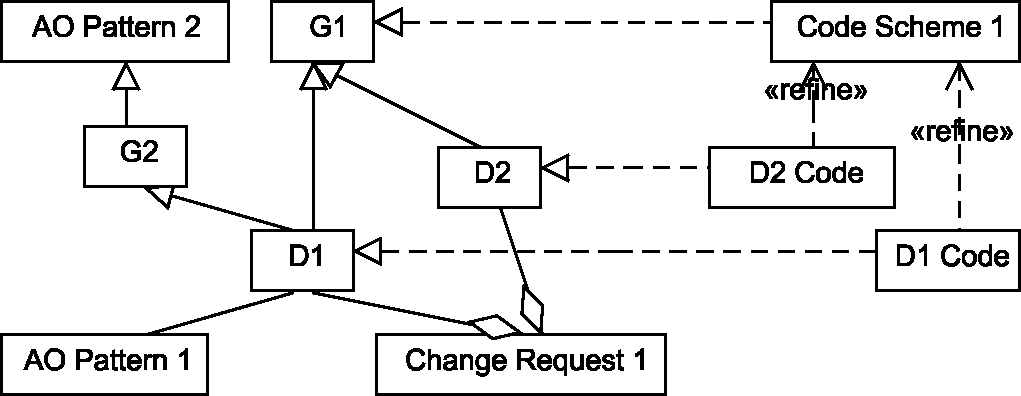
\includegraphics[scale=\magnf]{fig/gen-spec}
\caption{Generally applicable and domain specific changes.}
\label{f:gen-spec}
\end{figure}



\section{In� �as�} \label{ina}

V �asti~\ref{nejaka-pod} bol vysvetlen� princ�p~\cite{Vranic:AJParadigms,Alexander:Timeless}\ldots Toto je k�d:
\ajset
\begin{lstlisting}
public class SMTPServerM extends SMTPServer {
   . . .
}
. . .
public aspect SMTPServerBackupA {
   public pointcut SMTPServerConstructor(URL url, String user, String password):
      call(SMTPServer.new(..)) && args (url, user, password);
   SMTPServer around(URL url, String user, String password):
      SMTPServerConstructor(url, user, password) {
      return getSMTPServerBackup(proceed(url, user, password));
   }
   private SMTPServer getSMTPServerBackup(SMTPServer obj) {
      if (obj.isConnected()) {
         return obj;
      }
      else {
         return new SMTPServerM(obj.getUrl(), obj.getUser(),
            obj.getPassword());
      }
   }
}
\end{lstlisting}

     

\section{Zhodnotenie a a �al�ia pr�ca} \label{cc} 

\ldots


\bibliographystyle{abbrv} % m��e by� aj plain alebo alpha
\bibliography{mybib}

\appendix
\section{Nejak� pr�loha} \label{pnejaka}


\section{E�te nejak� pr�loha} \label{epnejaka}


\end{document}
